\documentclass[a4paper,12pt]{article} 

%%% Работа с русским языком
\usepackage{cmap}					% поиск в PDF
\usepackage{mathtext} 				% русские буквы в фомулах
\usepackage[T2A]{fontenc}			% кодировка
\usepackage[utf8]{inputenc}			% кодировка исходного текста
\usepackage[english,russian]{babel}	% локализация и переносы

%%% Дополнительная работа с математикой
\usepackage{amsmath,amsfonts,amssymb,amsthm,mathtools, gensymb} % AMS
\usepackage{icomma} % "Умная" запятая: $0,2$    ф--- число, $0, 2$ --- перечисление

%%Таблица
\usepackage[table,xcdraw]{xcolor}
\usepackage{caption}
\usepackage{floatrow}
\floatsetup[table]{capposition=top}
\floatsetup[wrapfigure]{capposition=bottom}

%Отступы и поля 
\textwidth=18cm
\oddsidemargin=-1cm
\topmargin=-2cm
\textheight=25cm


%% Номера формул
\mathtoolsset{showonlyrefs=true} % Показывать номера только у тех формул, на которые есть \eqref{} в тексте.

%% Шрифты
\usepackage{euscript}	 % Шрифт Евклид
\usepackage{mathrsfs} % Красивый матшрифт

%% Свои команды
\DeclareMathOperator{\sgn}{\mathop{sgn}}

%% Перенос знаков в формулах (по Львовскому)
\newcommand*{\hm}[1]{#1\nobreak\discretionary{}
{\hbox{$\mathsurround=0pt #1$}}{}}

%% Стиль страницы
\usepackage{fancyhdr}

%% Для рисунков
\usepackage{graphicx}
\usepackage[export]{adjustbox}
\usepackage{float}
\usepackage{ragged2e}
\usepackage{wrapfig}

\pagestyle{fancy}
\begin{document}
\begin{titlepage}
\begin{center}
%\vspace*{1cm}
\large{\small ФЕДЕРАЛЬНОЕ ГОСУДАРСТВЕННОЕ АВТОНОМНОЕ ОБРАЗОВАТЕЛЬНОЕ\\ УЧРЕЖДЕНИЕ ВЫСШЕГО ОБРАЗОВАНИЯ \\ МОСКОВСКИЙ ФИЗИКО-ТЕХНИЧЕСКИЙ ИНСТИТУТ\\ (НАЦИОНАЛЬНЫЙ ИССЛЕДОВАТЕЛЬСКИЙ УНИВЕРСИТЕТ)\\ ФАКУЛЬТЕТ АЭРОКОСМИЧЕСКИХ ТЕХНОЛОГИЙ}
\vfill
\line(1,0){490}\\[1mm]
\huge{Лабораторная работа 3.4.1}\\
\huge\textbf{Диа- и парамагнетики}\\
\line(1,0){490}\\[1mm]
\vfill
\begin{flushright}
\normalsize{Рогозин Владимир}\\
\normalsize{\textbf{Группа Б03-106}}\\
\end{flushright}
\end{center}
\end{titlepage}
\fancyhead[L] {Работа 3.4.1}


\textbf{Цель работы}: 
измерение магнитной восприимчивости диа- и парамагнитного образцов.

\textbf{Оборудование}: 
электромагнит, весы, милливеберметр, регулируемый источник постоянного тока, образцы диа- и пара-магнетиков.   

\textbf{Теоретические сведения}: 
Известно, что вещество может обладать как собственной намагниченностью, так и изменять свою намагниченность при помещении во внешнее магнитное поле. Микроскопическими источниками магнитного поля в среде являются орбитальное движение электронов в молекулах и атомах, а также собственное вращение (спин) электронов и ядер. При \textit{макроскопическом} описании свойств среды можно считать, что каждый элемент объёма среды может являться элементарным источником магнитного поля — \textit{магнитным диполем}.  Для описания усреднённых свойств среды используют вектор намагниченности \textit{\textbf{M}}, равный магнитному моменту единичного объёма вещества.

 Величина магнитного поля \textit{\textbf{B}} в данной точке среды определяется как значение микрополя, усреднённое по малому (элементарному) объёму, содержащему при этом большое количество частиц. \textit{\textbf{B}} называется индукцией магнитного поля.

 Помимо этого, принято вводить вспомогательный вектор \textit{\textbf{H}} напряженности поля.
\[\textit{\textbf{B}} = \textit{\textbf{H}} + 4\pi \textit{\textbf{M}}\]

В простейшем практически важном случае намагниченность \textit{\textbf{M}} в каждой точке среды прямо пропорциональна вектору напряжённости магнитного поля \textit{\textbf{H}} в этой же точке

\[\textit{\textbf{M}} = \chi \textit{\textbf{H}}\]
Коэффициент пропорциональности $\chi$ называется называют магнитной восприимчивостью среды. Вещества, для которых справедлива такая зависимость между намагниченностью и напряженностью, называются парамагнетиками ($\chi > 0$) и диамагнетиками ($\chi < 0$). В парамагнетиках элементарные диполи ориентированы в основном по приложенному полю, а в диамагнетиках -- против него.

В итоге для напряженности поля можем записать
\[\textit{\textbf{B}} = \mu\textit{\textbf{H}}\]
где $\mu$ -- магнитная проницаемость вещества
\[\mu = 1 + 4\pi \chi\]

\textbf{Диамагнетизм}

Диамагнетизм ($\chi$ < 0) возникает из-за электромагнитной индукции
молекулярных токов в электронных оболочках атомов и присущ в той
или иной степени всем веществам без исключения. В зависимости от
того, обладает ли электрон в атоме начальным моментом импульса \textit{\textbf{L}},
механизмы возникновения диамагнетизма несколько отличаются.

1) $\textit{\textbf{L}} = 0$. Рассмотрим электрон в состоянии с нулевым орбитальным моментом импульса. С классической точки зрения такое состояние можно представить как симметрично «размазанное» облако заряда вокруг ядра.

Плавно (квазистатически) включим внешнее однородное магнитное поле \textit{\textbf{B}}.  Согласно закону электромагнитной индукции, величина
этого поля на расстоянии $r$ от оси системы определяется соотношением
\[2\pi r E = -\pi r^2 \frac{dB}{dt}\]
отсюда 
\[E = -\frac{1}{2} r \frac{dB}{dt}\]
Запишем уравнение моментов для точечного электрона, находящегося
на «орбите» радиуса 
\[m_e r^2 \frac{d\omega}{dt} = -e r E = \frac{1}{2} e r^2 \frac{dB}{dt}\]
Интегрируя по времени, найдём, что независимо от расстояния $r$
электрон при включении поля $B$ приобретает угловую скорость вращения
\[\omega_L = \frac{e}{2m_e} B\]
Величину $\omega_L$ называют ларморовской частотой.

При вращении с ларморовской частотой электрон создаёт магнитное поле, равное полю витка с током $I_L = e  \frac{\omega_L}{2\pi}$. Этот ток в свою очередь
создаёт магнитный момент, по модулю равный
\[m_L = I_L \cdot S = -\frac{e^2 S}{4\pi m_e}B\]
где $S$ -- площадь эквивалентного витка. Если полагать, что $S \sim \pi a^2$, где $a$ -- среднее расстояние электронов до ядра. Тогда для атома, содержащего $Z$ электронов, иммем намагниченность среды $M = Z n \cdot \Delta m_L$, где $n$ есть число атомов в единице объёма. Получаем оценку для магнитной восприимчивости
\[\chi_{диа} \sim -\mu_0\frac{e^2 a^2}{4 m_e} Z n\]

2) $\textit{\textbf{L}} \neq 0$. Рассмотрим теперь случай, когда электрон исходно обладает некоторым орбитальным моментом импульса $L = mvr$. Орбитальное движение электрона эквивалентно витку с током, магнитный момент которого $m_L$ пропорционален $L$ и направлен против него. Его величину можно найти как
произведение тока $e \cdot \frac{v}{2 \pi r}$ на площадь «витка» $\pi r^2$: $m_L = \frac{1}{2} e v r$. При включении внешнего магнитного поля \textit{\textbf{B}}, направленного вдоль $z$, на электрон начинает действовать момент силы  $m_L \times B$, и уравнение движения электрона  будет иметь вид
\[\frac{dL}{dt} = m_L \times B\]

\begin{figure}[H]\label{fig: Прецессия электрона}
    \centering
    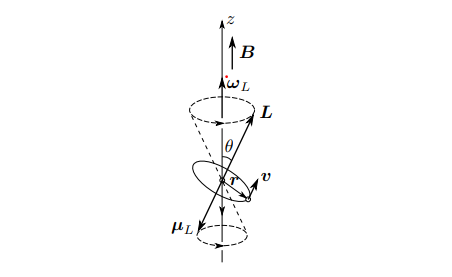
\includegraphics[width = 0.8 \textwidth]{Прецессия электрона.png}
    \caption{Прецессия электронной орбиты в магнитном поле}
\end{figure}
Его решением является прецессия электронной орбиты с ларморовской угловой частотой: $\omega_L = \frac{m_L}{L} B = \frac{e}{2 m_e}B$. При этом вектор $m_L$ описывает конус вокруг вектора $B$. Эта прецессия
не зависит от угла $\theta$ и приводит к дополнительному вращению электрона
вокруг поля $B$, налагающемуся на его орбитальное движение.

Отсюда следует, что диамагнитная восприимчивость не
зависит от температуры или величины поля и возрастает пропорционально порядковому номеру элемента. Видно, что диамагнитный эффект присущ всем веществам независимо от того, имеется у атомов собственный магнитный момент или нет. Однако у некоторых веществ он перекрывается более сильным парамагнитным эффектом.

\textbf{Парамагнетизм}

Парамагнетизм ($\chi$ > 0) характерен для веществ, микроскопические частицы которых (атомы, ионы, молекулы) обладают собственным магнитным моментом в отсутствие внешнего магнитного поля. 

В парамагнетиках энергия взаимодействия между соседними магнитными моментами атомов мала по сравнению с тепловой энергией, поэтому в отсутствие внешнего магнитного поля микроскопические магнитные моменты полностью разупорядочены, и намагниченность среды равна нулю. При помещении во внешнее поле магнитным моментам энергетически выгодно ориентироваться преимущественно по полю, что и приводит к парамагнитному эффекту.

Оценим температурную зависимость магнитной восприимчивости парамагнетика в классической модели.  Пусть среднее число атомов в единице объёма равно $n$, а абсолютная величина магнитного момента атома $\mathfrak{m}_a$. В магнитном поле с индукцией $B$ энергия магнитного диполя, составляющего с направлением поля угол $\alpha$, равна
\[U = -\mathfrak{m}_a B \cos \alpha\]
и может меняться в диапазоне от $ -\mathfrak{m}_a B \cos \alpha$ до $\mathfrak{m}_a B \cos \alpha $

Из термодинамики известно, что доля атомов $dn$, обладающих в условиях равновесия энергией $U(\alpha)$, определяется распределением Больцмана:
\[dn \propto e^{- \frac{U(\alpha)}{k_{Б} T}}d\alpha\]
Пусть внешнее магнитное поле достаточно мало, так что энергия магнитных моментов атомов в нём много меньше тепловой: $\mathfrak{m}_a B \ll k_{Б} T$. Число
атомов, имеющих положительную ($\alpha$ > 0) проекцию на направление $B$, может быть записано как
\[n_{+} = n_0 e^{\mathfrak{m}_a B / k_{Б} T} \approx n_0 \Big(1 + \frac{\mathfrak{m}_a B}{k_{Б} T}\Big)\]
 Для атомов с отрицательной проекцией момента ($\alpha$ < 0)
 \[n_{-} = n_0 e^{\mathfrak{m}_a B / k_{Б} T} \approx n_0 \Big(1 - \frac{\mathfrak{m}_a B}{k_{Б} T}\Big)\]
Учитывая условие нормировки $n_{+} + n_{-} = n$, найдём: $n_0 \approx n / 2$.

Величину суммарного магнитного момента единицы объёма можно оценить как
\[M \sim n_{+} \mathfrak{m}_a + n_{-} (-\mathfrak{m}_a) \approx \frac{\mathfrak{m}_a^2 n }{k_{Б} T} B\]
Более аккуратное усреднение по углам даст поправочный множитель порядка единицы (в классической модели получается коэффициент $1 / 3$).

Таким образом, парамагнитная восприимчивость равна
\[\chi_{пар} \sim \mu_0 \frac{\mathfrak{m}_a^2 n }{3 k_{Б} T} \propto \frac{1}{T}\]
Температурная зависимость восприимчивости парамагнетиков называется \textit{законом Кюри}.

\begin{wrapfigure}[11]{r}{0.45\textwidth}\label{fig: образец в поле}
    \begin{center}
    \vspace{-30pt}
        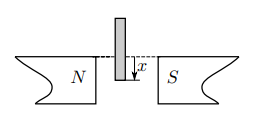
\includegraphics[width = \textwidth]{Образец в зазоре.png}
    \end{center}
    \caption{Расположение образца в зазоре электромагнита}
\end{wrapfigure}

\textbf{Методика измерения}:
Магнитная восприимчивость тел может быть определена по измерению сил, действующих на тела в магнитном поле. Существуют два классических метода таких измерений: \textit{метод Фарадея} и \textit{метод Гюи}. В данной работе предлагается использовать метод Гюи. В методе Гюи используется тонкий и длинный стержень, один из концов которого помещают в зазор электромагнита (обычно в область однородного поля), а другой конец -- вне зазора, где величиной магнитного поля можно пренебречь. Закон изменения поля — от максимального до нулевого — в этом случае несуществен. 

Найдём выражение для силы, действующей со стороны магнитного поля на цилиндрический стержень, помещённый в зазор электромагнита (рис. 1). Пусть
площадь сечения образца равна $S$, его магнитная проницаемость -- $\mu$, поле в зазоре равно $B_0$ и образец помещён в зазор на глубину $x$.

Ток в обмотке электромагнита $I$ поддерживается постоянным, поэтому сила, действующая на образец со стороны магнитного поля равна
\[F_M = \Big( \frac{\partial W_M}{\partial x}\Big)\]
где $W_M(x)$ -- магнитная энергия системы при $I = const$ в зависимости от смещения образца $x$.

Магнитная энергия может быть рассчитана по формуле:
\[W_M = \frac{1}{2\mu_0} \int \frac{B^2}{\mu} dV\]
где интегрирование проводится по всему пространству.

Найдём распределение магнитного поля в длинном цилиндре, частично помещённом в зазор электромагнита.
\begin{wrapfigure}[13]{r}{0.5\textwidth}\label{fig: расчет силы}
    \begin{center}
    \vspace{-110pt}
        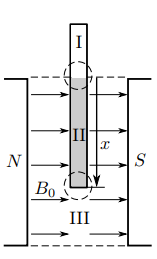
\includegraphics[width = 0.5\textwidth]{Для расчета силы.png}
    \end{center}
    \caption{К вычислению распределения
поля в образце}
\end{wrapfigure}

Систему можно условно разбить на 3 части. В области $I$ вне электромагнита поле мало
 $B_1 \approx 0$ и его вкладом в энергию можно пренебречь. В части стержня $II$, погружённой в электромагнит, поле приближённо равно $B_2 \approx \mu B_0$. В области $III$ вдали от стержня поле мало отличается от $B_3 \approx B_0$. Наконец, в пограничных областях между $I$ и $II$ и между $II$ и $III$ (отмечены пунктиром) распределение поля простыми методами рассчитано быть не может. Найдём изменение магнитной энергии при заданном
смещении:
\[dW_M(\Delta x) \approx \frac{B_2^2}{2\mu \mu_0} S dx - \frac{B_3^2}{2\mu_0} S dx = (\mu - 1)\frac{B_0^2}{2\mu_0} S dx\]
Отсюда, сила равна
\[F_M = \Big( \frac{\partial W_M}{\partial x}\Big)_{B_0} \approx \chi \frac{B_0^2}{2\mu_0} S\]
Знак силы зависит от знака восприимчивости, парамагнетики ($\chi$ > 0) втягиваются в зазор электромагнита, а диамагнетики ($\chi$ < 0) выталкиваются из него. 

\textbf{Экспериментальная установка}:
\begin{figure}[H]\label{fig: ustanovka}
    \centering
    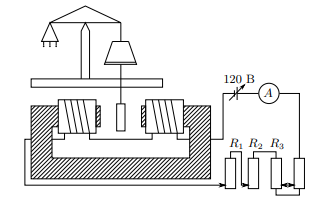
\includegraphics[width = 0.7 \textwidth]{Установка.png}
    \caption{Схема экспериментальной установки}
\end{figure}

Схема установки изображена на рис. 4. Магнитное поле с максимальной индукцией $\approx$ 1 Тл создаётся в зазоре электромагнита, питаемого
постоянным током. Диаметр полюсов существенно превосходит ширину зазора, поэтому поле в средней части зазора достаточно однородно. Величина тока, проходящего через обмотки электромагнита, задаётся регулируемым источником постоянного напряжения.

Градуировка электромагнита (связь между индукцией магнитного поля $B$ в зазоре электромагнита и силой тока $I$ в его обмотках) производится при помощи милливеберметра.

При измерениях образцы поочерёдно подвешиваются к аналитическим весам так, что один конец образца оказывается в зазоре электромагнита, а другой — вне зазора, где индукцией магнитного поля можно пренебречь. При помощи аналитических весов определяется перегрузка  $\Delta P = F$ -- сила, действующая на образец со стороны магнитного поля.

Cилы, действующие на диа- и парамагнитные
образцы, очень малы. Небольшие примеси ферромагнетиков (сотые доли процента железа или никеля) способны кардинально изменить результат
опыта, поэтому образцы были специально отобраны.


\textbf{Обработка данных}:  Сначала прокалибруем электромагнит, для этого  с помощью милливеберметра снимем зависимость магнитного потока $\Phi$,  пронизывающего пробную катушку, находящуюся в зазоре, от тока $I$. Таким образом наёдем зависимость $B(I)$ ($\Phi = B S N$), где $SN = 72 \text{ } см^2$. Данные для калибровки представлены ниже в таблице:

\begin{table}[H]\label{tab: Phi ot I}
    \centering
    \begin{tabular}{|c|c|c|c|}
        \hline
        {\color[HTML]{000000} $I$, A} & {\color[HTML]{000000} $\Phi$, мВб} & {\color[HTML]{000000} $I$, A} & {\color[HTML]{000000} $\Phi$, мВб} \\ \hline
        {\color[HTML]{000000} 0,3} & {\color[HTML]{000000} 0,75} & {\color[HTML]{000000} 1,8} & {\color[HTML]{000000} 3,9}  \\ \hline
        {\color[HTML]{000000} 0,6} & {\color[HTML]{000000} 1,3}  & {\color[HTML]{000000} 2,1} & {\color[HTML]{000000} 4,5}  \\ \hline
        {\color[HTML]{000000} 0,9} & {\color[HTML]{000000} 2}    & {\color[HTML]{000000} 2,4} & {\color[HTML]{000000} 5,05} \\ \hline
        {\color[HTML]{000000} 1,2} & {\color[HTML]{000000} 2,7}  & {\color[HTML]{000000} 2,7} & {\color[HTML]{000000} 5,6}  \\ \hline
        {\color[HTML]{000000} 1,5} & {\color[HTML]{000000} 3,3}  & {\color[HTML]{000000} 3,0} & {\color[HTML]{000000} 6}    \\ \hline
    \end{tabular}
    \caption{Данные для калибровки электромагнита}
\end{table}

Внешнее сопротивление цепи равно $r_{внеш} = 5$ Ом, при таком сопротивлении относительная погрешность измерения потока не превышает $\varepsilon_{\Phi} = 1,5 \%$. Погрешность измерения силы тока не превышает $0,5 \%$ + 2 единицы младшего разряда (0,01 А). По значениям из таблице выше построим график зависимости $B (I)$.

\begin{figure}[H]\label{fig: B(I)}
    \centering
    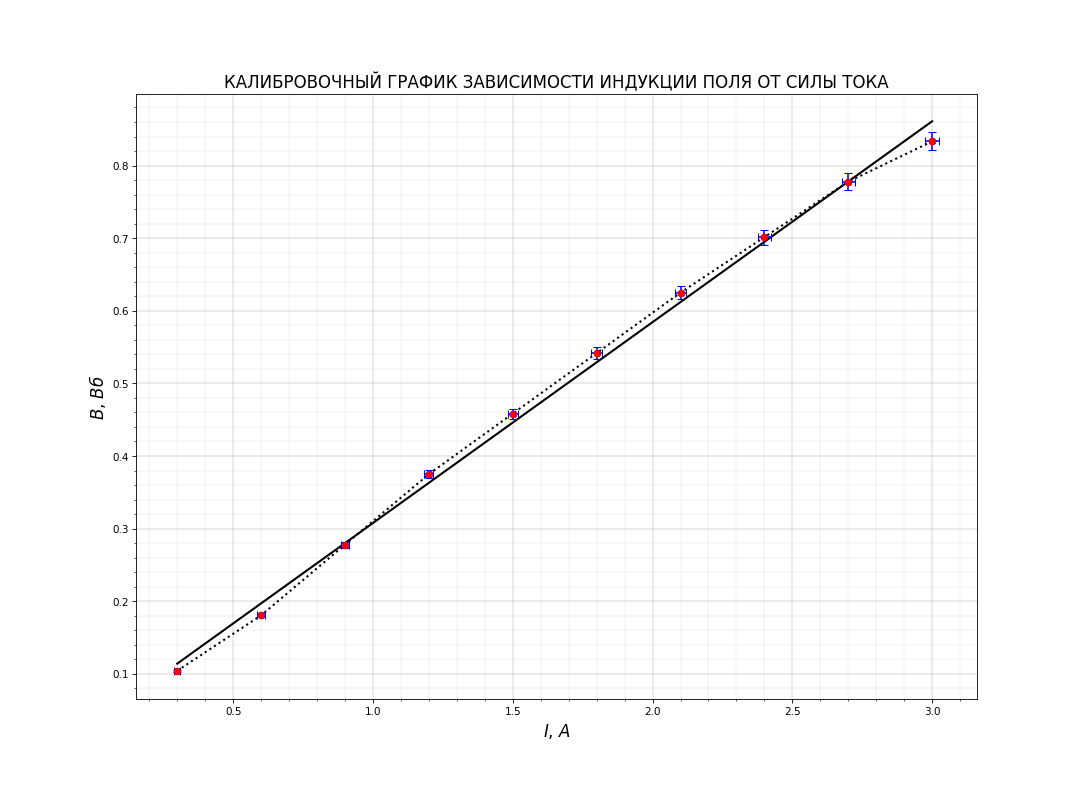
\includegraphics[width =  1\textwidth]{B(I).png}
\end{figure}
\[k = (276,65 \pm 4,92) \text{ мВб/А,} \quad \varepsilon_{k} = 1,78 \%\]
\[b = (31,01 \pm 4,24) \text{ мВб,} \quad \varepsilon_{b} = 13,69 \%\]

Теперь, с помощью весов, измерим силу, действующую каждый из образцов, при разлтичных значениях силы тока $I$ в катушке (а следовательно и различных значениях индукции $B$). Причём снимем значения силы при увеличении силы тока, а затем при уменьшении, то есть идя в обратную сторону. Всего в работе использовались четыре образца из различных металлов. Данные по каждому из них представлены в таблицах ниже, абсолютная погрешность измерения диаметра образцов равна $\sigma_{d} = 0,1$ мм.

\begin{table}[H]\label{tab: Params of obrazec}
    \centering
    \begin{tabular}{|c|cccc|}
        \hline
        {\color[HTML]{000000} } & \multicolumn{4}{c|}{{\color[HTML]{000000} Образец}} \\ \hline
        {\color[HTML]{000000} $I$, A} &
          \multicolumn{1}{c|}{{\color[HTML]{000000} Al}} &
          \multicolumn{1}{c|}{{\color[HTML]{000000} Cu}} &
          \multicolumn{1}{c|}{{\color[HTML]{000000} C}} &
          {\color[HTML]{000000} W} \\ \hline
        {\color[HTML]{000000} $m,$ г} &
          \multicolumn{1}{c|}{{\color[HTML]{000000} 25,305}} &
          \multicolumn{1}{c|}{{\color[HTML]{000000} 83353}} &
          \multicolumn{1}{c|}{{\color[HTML]{000000} 11,859}} &
          {\color[HTML]{000000} 13,843} \\ \hline
        {\color[HTML]{000000} $d,$ мм} &
          \multicolumn{1}{c|}{{\color[HTML]{000000} 10,0}} &
          \multicolumn{1}{c|}{{\color[HTML]{000000} 10,0}} &
          \multicolumn{1}{c|}{{\color[HTML]{000000} 10,0}} &
          {\color[HTML]{000000} 3,1} \\ \hline
    \end{tabular}
    \caption{Параметры образцов}
\end{table}

\begin{table}[H]\label{tab: F ot I}
    \centering
    \begin{tabular}{|c|cccccccc|}
        \hline
        {\color[HTML]{000000} } &
          \multicolumn{1}{c|}{{\color[HTML]{000000} Al,  up}} &
          \multicolumn{1}{c|}{{\color[HTML]{000000} Al,  down}} &
          \multicolumn{1}{c|}{{\color[HTML]{000000} Cu,  up}} &
          \multicolumn{1}{c|}{{\color[HTML]{000000} Cu,  down}} &
          \multicolumn{1}{c|}{{\color[HTML]{000000} C,  up}} &
          \multicolumn{1}{c|}{{\color[HTML]{000000} C,  down}} &
          \multicolumn{1}{c|}{{\color[HTML]{000000} W,  up}} &
          {\color[HTML]{000000} W,  down} \\ \hline
        {\color[HTML]{000000} $I$, A} &
          \multicolumn{8}{c|}{{\color[HTML]{000000} $\Delta P$, мг}} \\ \hline
        {\color[HTML]{000000} 0,3} &
          \multicolumn{1}{c|}{{\color[HTML]{000000} 0}} &
          \multicolumn{1}{c|}{{\color[HTML]{000000} 2}} &
          \multicolumn{1}{c|}{{\color[HTML]{000000} 0}} &
          \multicolumn{1}{c|}{{\color[HTML]{000000} 0}} &
          \multicolumn{1}{c|}{{\color[HTML]{000000} -14}} &
          \multicolumn{1}{c|}{{\color[HTML]{000000} -18}} &
          \multicolumn{1}{c|}{{\color[HTML]{000000} 0}} &
          {\color[HTML]{000000} 0} \\ \hline
        {\color[HTML]{000000} 0,6} &
          \multicolumn{1}{c|}{{\color[HTML]{000000} 2}} &
          \multicolumn{1}{c|}{{\color[HTML]{000000} 4}} &
          \multicolumn{1}{c|}{{\color[HTML]{000000} 0}} &
          \multicolumn{1}{c|}{{\color[HTML]{000000} -1}} &
          \multicolumn{1}{c|}{{\color[HTML]{000000} -36}} &
          \multicolumn{1}{c|}{{\color[HTML]{000000} -44}} &
          \multicolumn{1}{c|}{{\color[HTML]{000000} 0}} &
          {\color[HTML]{000000} 0} \\ \hline
        {\color[HTML]{000000} 0,9} &
          \multicolumn{1}{c|}{{\color[HTML]{000000} 5}} &
          \multicolumn{1}{c|}{{\color[HTML]{000000} 7}} &
          \multicolumn{1}{c|}{{\color[HTML]{000000} 0}} &
          \multicolumn{1}{c|}{{\color[HTML]{000000} -2}} &
          \multicolumn{1}{c|}{{\color[HTML]{000000} -68}} &
          \multicolumn{1}{c|}{{\color[HTML]{000000} -72}} &
          \multicolumn{1}{c|}{{\color[HTML]{000000} 0}} &
          {\color[HTML]{000000} 1} \\ \hline
        {\color[HTML]{000000} 1,2} &
          \multicolumn{1}{c|}{{\color[HTML]{000000} 9}} &
          \multicolumn{1}{c|}{{\color[HTML]{000000} 11}} &
          \multicolumn{1}{c|}{{\color[HTML]{000000} -2}} &
          \multicolumn{1}{c|}{{\color[HTML]{000000} -3}} &
          \multicolumn{1}{c|}{{\color[HTML]{000000} -96}} &
          \multicolumn{1}{c|}{{\color[HTML]{000000} -100}} &
          \multicolumn{1}{c|}{{\color[HTML]{000000} 1}} &
          {\color[HTML]{000000} 1} \\ \hline
        {\color[HTML]{000000} 1,5} &
          \multicolumn{1}{c|}{{\color[HTML]{000000} 14}} &
          \multicolumn{1}{c|}{{\color[HTML]{000000} 17}} &
          \multicolumn{1}{c|}{{\color[HTML]{000000} -4}} &
          \multicolumn{1}{c|}{{\color[HTML]{000000} -5}} &
          \multicolumn{1}{c|}{{\color[HTML]{000000} -122}} &
          \multicolumn{1}{c|}{{\color[HTML]{000000} -129}} &
          \multicolumn{1}{c|}{{\color[HTML]{000000} 2}} &
          {\color[HTML]{000000} 2} \\ \hline
        {\color[HTML]{000000} 1,8} &
          \multicolumn{1}{c|}{{\color[HTML]{000000} 20}} &
          \multicolumn{1}{c|}{{\color[HTML]{000000} 22}} &
          \multicolumn{1}{c|}{{\color[HTML]{000000} -6}} &
          \multicolumn{1}{c|}{{\color[HTML]{000000} -8}} &
          \multicolumn{1}{c|}{{\color[HTML]{000000} -149}} &
          \multicolumn{1}{c|}{{\color[HTML]{000000} -156}} &
          \multicolumn{1}{c|}{{\color[HTML]{000000} 4}} &
          {\color[HTML]{000000} 4} \\ \hline
        {\color[HTML]{000000} 2,1} &
          \multicolumn{1}{c|}{{\color[HTML]{000000} 27}} &
          \multicolumn{1}{c|}{{\color[HTML]{000000} 29}} &
          \multicolumn{1}{c|}{{\color[HTML]{000000} -10}} &
          \multicolumn{1}{c|}{{\color[HTML]{000000} -11}} &
          \multicolumn{1}{c|}{{\color[HTML]{000000} -176}} &
          \multicolumn{1}{c|}{{\color[HTML]{000000} -182}} &
          \multicolumn{1}{c|}{{\color[HTML]{000000} 7}} &
          {\color[HTML]{000000} 7} \\ \hline
        {\color[HTML]{000000} 2,4} &
          \multicolumn{1}{c|}{{\color[HTML]{000000} 34}} &
          \multicolumn{1}{c|}{{\color[HTML]{000000} 36}} &
          \multicolumn{1}{c|}{{\color[HTML]{000000} -12}} &
          \multicolumn{1}{c|}{{\color[HTML]{000000} -15}} &
          \multicolumn{1}{c|}{{\color[HTML]{000000} -199}} &
          \multicolumn{1}{c|}{{\color[HTML]{000000} -206}} &
          \multicolumn{1}{c|}{{\color[HTML]{000000} 9}} &
          {\color[HTML]{000000} 10} \\ \hline
        {\color[HTML]{000000} 2,7} &
          \multicolumn{1}{c|}{{\color[HTML]{000000} 42}} &
          \multicolumn{1}{c|}{{\color[HTML]{000000} 43}} &
          \multicolumn{1}{c|}{{\color[HTML]{000000} -16}} &
          \multicolumn{1}{c|}{{\color[HTML]{000000} -18}} &
          \multicolumn{1}{c|}{{\color[HTML]{000000} -221}} &
          \multicolumn{1}{c|}{{\color[HTML]{000000} -225}} &
          \multicolumn{1}{c|}{{\color[HTML]{000000} 12}} &
          {\color[HTML]{000000} 12} \\ \hline
        {\color[HTML]{000000} 3,0} &
          \multicolumn{1}{c|}{{\color[HTML]{000000} 48}} &
          \multicolumn{1}{c|}{{\color[HTML]{000000} 48}} &
          \multicolumn{1}{c|}{{\color[HTML]{000000} -19}} &
          \multicolumn{1}{c|}{{\color[HTML]{000000} -21}} &
          \multicolumn{1}{c|}{{\color[HTML]{000000} -239}} &
          \multicolumn{1}{c|}{{\color[HTML]{000000} -239}} &
          \multicolumn{1}{c|}{{\color[HTML]{000000} 14}} &
          {\color[HTML]{000000} 14} \\ \hline
    \end{tabular}
    \caption{Данные для построения графиков зависимости}
\end{table}

По данным из таблицы построим графики зависимости $\Delta P$ от $B^2$, где значение $\Delta P$ берётся среднее арифметическое двух (вверх и вниз). Абсолютная погрешность измерения $\Delta P$ равна $\sigma_{\Delta P } = 1$ мг.

\begin{figure}[H]\label{fig: Al_Cu}
    \centering
    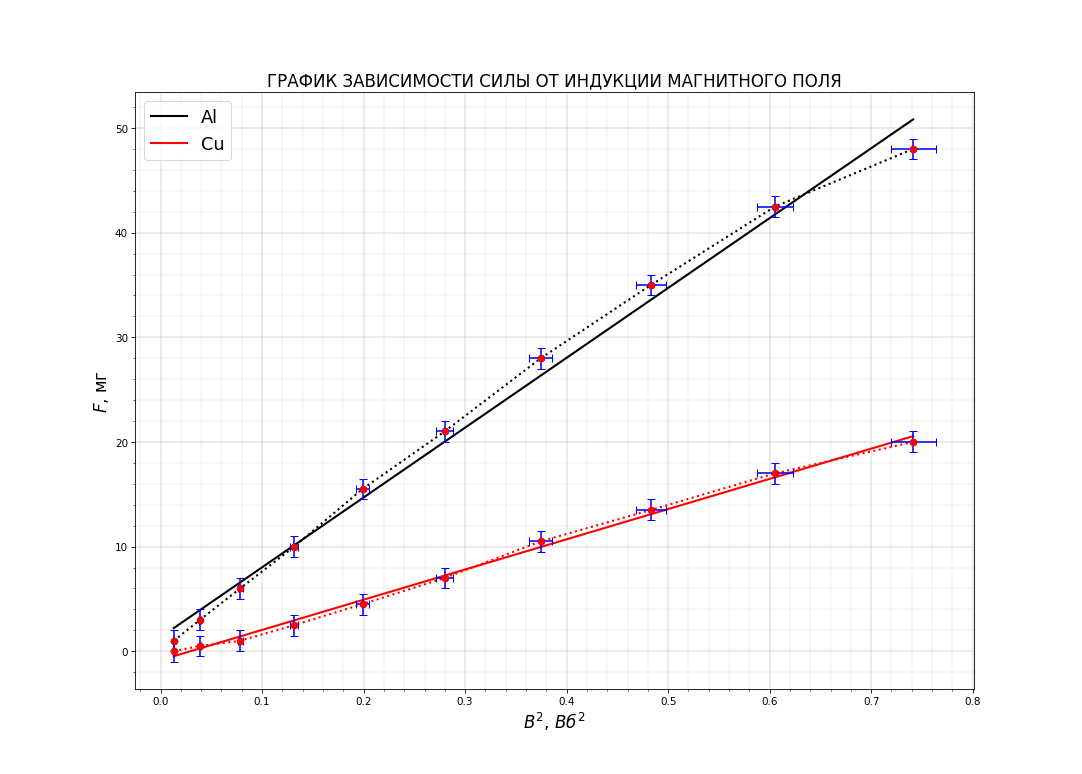
\includegraphics[width = \textwidth]{F(B2)Al_Cu.png}
\end{figure}

\[k_{Al} = (66,75 \pm 1,77) \text{ мг/$Тл^2$,} \quad \varepsilon_{k} = 2,65 \%\]
\[k_{Cu} = (28,87 \pm 0,56) \text{ мг/$Тл^2$,} \quad \varepsilon_{k} = 1,93 \%\]

Для меди и алюминия рассчитаем магнитную восприимчивость
\[ \fbox{$\chi = 2 k \cdot \frac{\mu_0}{S}$} \]
где $S$ -- площадь поперечного сечения образца $S =\pi d^2 / 4$, $\mu_0$ -- магнитная постоянная.
\[\chi_{Al} = (21,41 \pm 0,71) \cdot 10^{-6}, \quad \varepsilon_{\chi} = 3,32\%\]
\[\chi_{Cu} = (-9,26 \pm 0,36) \cdot 10^{-6}, \quad \varepsilon_{\chi} = 2,78\%\]
Относительная погрешность магнитной восприимчивости была найдена по формуле
\[\varepsilon_{\chi}^2 = \varepsilon_k^2 + 4\varepsilon_d^2\]

Сравним полученные значения с табличными: $\chi_{Al \text{ }табл} = 23 \cdot 10^{-6}$, полученное для алюминия значение отличается от табличного на $\sim 7\%$; $\chi_{Cu \text{ }табл} = -1 \cdot 10^{-5}$, для меди результат отличается от табличного также на $\sim 7 \%$.

Далее построим аналогичные графики и рассчитаем магнитную восприимчивость для образцов из вольфрама и графита.

\begin{figure}[H]\label{fig: W}
    \centering
    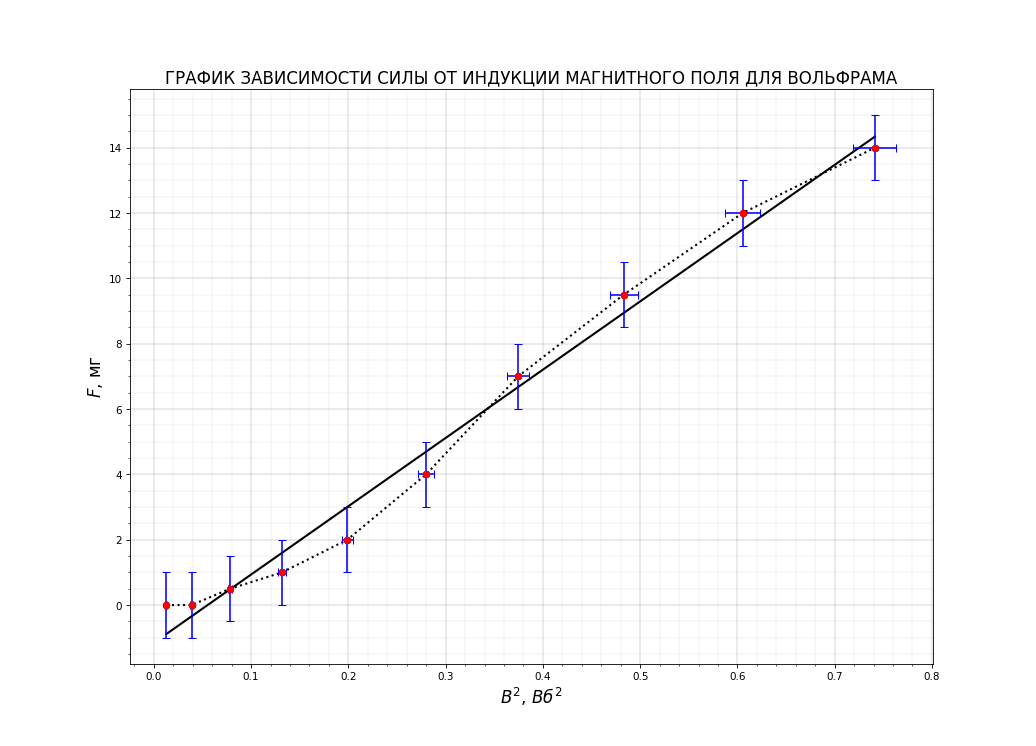
\includegraphics[width = \textwidth]{F(B2)W.png}
\end{figure}
\[k_{W} = (20,90 \pm 0,79) \text{ мг/$Тл^2$,} \quad \varepsilon_{k} = 3,78 \%\]
\[\chi_{W} = (69,78 \pm 2,99) \cdot 10^{-6}, \quad \varepsilon_{\chi} = 4,28\%\]
Табличое значение магнитной вопсприимчивости для вольфрама $\chi_{W \text{ }табл} = 55 \cdot 10^{-6}$, полученная на опыте величина отличается на $\sim 27\%$.

Далее найдём $\chi$ для материала последнего образца -- графита.

\begin{figure}[H]\label{fig: C}
    \centering
    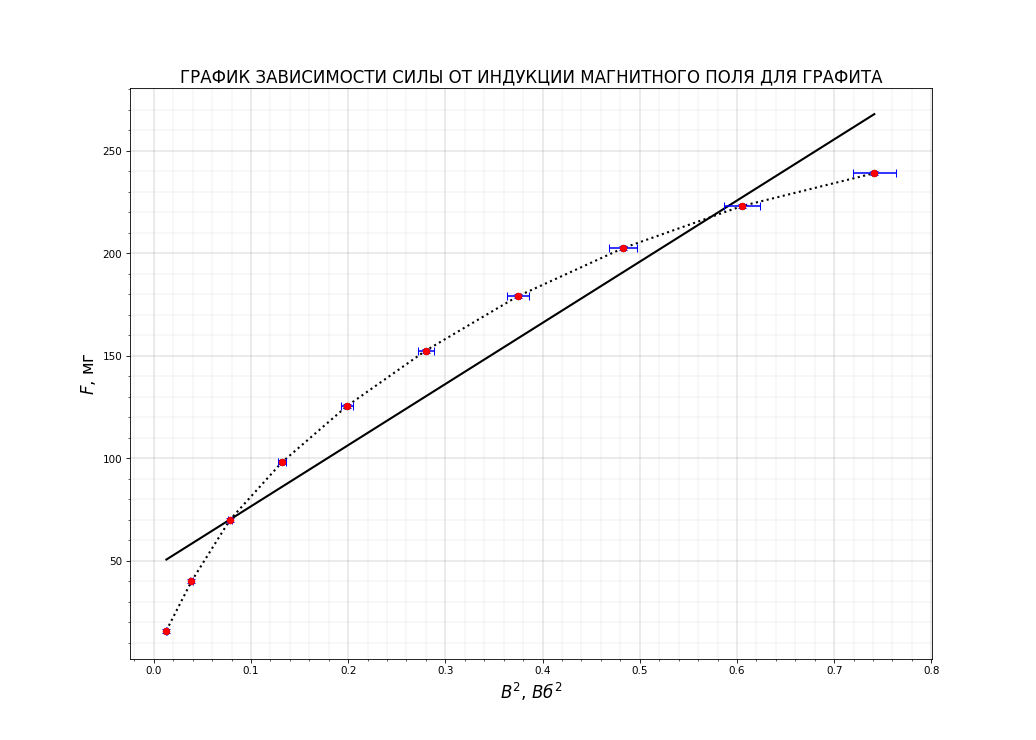
\includegraphics[width = \textwidth]{F(B2)С.png}
\end{figure}
\[k_{C} = (298,20 \pm 26,48) \text{ мг/$Тл^2$,} \quad \varepsilon_{k} = 8,88 \%\]
\[\chi_{C} = (95,68 \pm 8,71) \cdot 10^{-6}, \quad \varepsilon_{\chi} = 9,10\%\]
Табличое значение магнитной восприимчивости графита $\chi_{C \text{ }табл} =  85 \cdot 10^{-6}$ отличается от $\chi_{эксп}$ на $\sim 13 \%$.

Занесём все результаты в таблицу и проанализируем их.
\begin{table}[H]\label{tab: chi result}
    \centering
    \begin{tabular}{|
        >{\columncolor[HTML]{ffffff}}c |
        >{\columncolor[HTML]{ffffff}}c |
        >{\columncolor[HTML]{ffffff}}c |
        >{\columncolor[HTML]{ffffff}}c |
        >{\columncolor[HTML]{ffffff}}c |}
        \hline
        {\color[HTML]{000000} Материал} &
          {\color[HTML]{000000} Алюминий} &
          {\color[HTML]{000000} Медь} &
          {\color[HTML]{000000} Вольфрам} &
          {\color[HTML]{000000} Графит} \\ \hline
        {\color[HTML]{000000} $\chi_{табл} \cdot 10^{6}$} &
          {\color[HTML]{000000} 23,0} &
          {\color[HTML]{000000} -9,26} &
          {\color[HTML]{000000} 55} &
          {\color[HTML]{000000} 85} \\ \hline
        {\color[HTML]{000000} $\chi_{эксп} \cdot 10^{6}$} &
          {\color[HTML]{000000} 21,41} &
          {\color[HTML]{000000} -10} &
          {\color[HTML]{000000} 69,78} &
          {\color[HTML]{000000} 95,68} \\ \hline
        {\color[HTML]{000000} $\varepsilon_{\chi_{эксп}}$, $\%$} &
          {\color[HTML]{000000} 3,32} &
          {\color[HTML]{000000} 2,78} &
          {\color[HTML]{000000} 4,28} &
          {\color[HTML]{000000} 9,10} \\ \hline
        {\color[HTML]{000000} Различие, $\%$} &
          {\color[HTML]{000000} 6,91} &
          {\color[HTML]{000000} 7,4} &
          {\color[HTML]{000000} 26,87} &
          {\color[HTML]{000000} 12,56} \\ \hline
    \end{tabular}
    \caption{Результаты вычислений}
\end{table}

\textbf{Вывод:} В данной работе были исследованы пара- и диамагнитные свойства меди, алюминия, вольфрама и графита, а также были вычислены значения магнитной восприимчивости для каждого из материалов. Результаты эксперимента неплохо совпали с теорией для алюминия и меди (отличие $\sim 7\%$), совпали хуже для графита ($\sim 13\%$) и гораздо хуже для вольфрама ($\sim 27\%$).

\end{document}
